\documentclass[]{article}
\usepackage{lmodern}
\usepackage{amssymb,amsmath}
\usepackage{ifxetex,ifluatex}
\usepackage{fixltx2e} % provides \textsubscript
\ifnum 0\ifxetex 1\fi\ifluatex 1\fi=0 % if pdftex
  \usepackage[T1]{fontenc}
  \usepackage[utf8]{inputenc}
\else % if luatex or xelatex
  \ifxetex
    \usepackage{mathspec}
  \else
    \usepackage{fontspec}
  \fi
  \defaultfontfeatures{Ligatures=TeX,Scale=MatchLowercase}
\fi
% use upquote if available, for straight quotes in verbatim environments
\IfFileExists{upquote.sty}{\usepackage{upquote}}{}
% use microtype if available
\IfFileExists{microtype.sty}{%
\usepackage{microtype}
\UseMicrotypeSet[protrusion]{basicmath} % disable protrusion for tt fonts
}{}
\usepackage[margin=1in]{geometry}
\usepackage{hyperref}
\hypersetup{unicode=true,
            pdftitle={The utility of spatial model-based estimators of unobserved bycatch: future or folly?},
            pdfauthor={Brian C. Stock1, Eric J. Ward2, James T. Thorson3, Jason E. Jannot3, Brice X. Semmens1},
            pdfborder={0 0 0},
            breaklinks=true}
\urlstyle{same}  % don't use monospace font for urls
\usepackage{graphicx,grffile}
\makeatletter
\def\maxwidth{\ifdim\Gin@nat@width>\linewidth\linewidth\else\Gin@nat@width\fi}
\def\maxheight{\ifdim\Gin@nat@height>\textheight\textheight\else\Gin@nat@height\fi}
\makeatother
% Scale images if necessary, so that they will not overflow the page
% margins by default, and it is still possible to overwrite the defaults
% using explicit options in \includegraphics[width, height, ...]{}
\setkeys{Gin}{width=\maxwidth,height=\maxheight,keepaspectratio}
\IfFileExists{parskip.sty}{%
\usepackage{parskip}
}{% else
\setlength{\parindent}{0pt}
\setlength{\parskip}{6pt plus 2pt minus 1pt}
}
\setlength{\emergencystretch}{3em}  % prevent overfull lines
\providecommand{\tightlist}{%
  \setlength{\itemsep}{0pt}\setlength{\parskip}{0pt}}
\setcounter{secnumdepth}{0}
% Redefines (sub)paragraphs to behave more like sections
\ifx\paragraph\undefined\else
\let\oldparagraph\paragraph
\renewcommand{\paragraph}[1]{\oldparagraph{#1}\mbox{}}
\fi
\ifx\subparagraph\undefined\else
\let\oldsubparagraph\subparagraph
\renewcommand{\subparagraph}[1]{\oldsubparagraph{#1}\mbox{}}
\fi

%%% Use protect on footnotes to avoid problems with footnotes in titles
\let\rmarkdownfootnote\footnote%
\def\footnote{\protect\rmarkdownfootnote}

%%% Change title format to be more compact
\usepackage{titling}

% Create subtitle command for use in maketitle
\newcommand{\subtitle}[1]{
  \posttitle{
    \begin{center}\large#1\end{center}
    }
}

\setlength{\droptitle}{-2em}

  \title{The utility of spatial model-based estimators of unobserved bycatch:
future or folly?}
    \pretitle{\vspace{\droptitle}\centering\huge}
  \posttitle{\par}
    \author{Brian C. Stock\textsuperscript{1}, Eric J. Ward\textsuperscript{2},
James T. Thorson\textsuperscript{3}, Jason E. Jannot\textsuperscript{3},
Brice X. Semmens\textsuperscript{1}}
    \preauthor{\centering\large\emph}
  \postauthor{\par}
    \date{}
    \predate{}\postdate{}
  
\usepackage{setspace}
%\singlespacing
%\onehalfspacing
\doublespacing
\usepackage{lineno}
\linenumbers
\usepackage{pdflscape}
\newcommand{\blandscape}{\begin{landscape}}
\newcommand{\elandscape}{\end{landscape}}
\usepackage{graphicx}
\usepackage{booktabs}
\usepackage{booktabs}
\usepackage{longtable}
\usepackage{array}
\usepackage{multirow}
\usepackage[table]{xcolor}
\usepackage{wrapfig}
\usepackage{float}
\usepackage{colortbl}
\usepackage{pdflscape}
\usepackage{tabu}
\usepackage{threeparttable}
\usepackage{threeparttablex}
\usepackage[normalem]{ulem}
\usepackage{makecell}

\begin{document}
\maketitle

\(^1\)+1 425 919 7879,
\href{mailto:b1stock@ucsd.edu}{\nolinkurl{b1stock@ucsd.edu}},
\href{mailto:semmens@ucsd.edu}{\nolinkurl{semmens@ucsd.edu}}, Scripps
Institution of Oceanography, University of California, San Diego, La
Jolla, California 92093 USA\\
\(^2\)\href{mailto:eric.ward@noaa.gov}{\nolinkurl{eric.ward@noaa.gov}},
Conservation Biology Division, Northwest Fisheries Science Center,
National Marine Fisheries Service, National Oceanic and Atmospheric
Administration, 2725 Montlake Blvd E, Seattle WA, 98112, USA\\
\(^3\)\href{mailto:james.thorson@noaa.gov}{\nolinkurl{james.thorson@noaa.gov}},
\href{mailto:jason.jannot@noaa.gov}{\nolinkurl{jason.jannot@noaa.gov}},
Fisheries Resource and Monitoring Division, Northwest Fisheries Science
Center, National Marine Fisheries Service, National Oceanic and
Atmospheric Administration, 2725 Montlake Blvd E, Seattle WA, 98112,
USA\\

\subsection{Abstract}\label{abstract}

Quantifying effects of fishing on non-targeted (bycatch) species is an
important management and conservation issue. Bycatch estimates are
typically calculated using data collected by on-board observers, but
observer programs are costly and therefore often only cover a small
percentage of the fishery. The challenge is then to estimate bycatch for
the unobserved fishing activity. The status quo for most fisheries is to
assume the ratio of bycatch-to-effort is constant and multiply this
ratio times the effort in the unobserved activity (ratio estimator). We
used a dataset with 100\% observer coverage, 35,440 hauls from the U.S.
West Coast groundfish trawl fishery, to evaluate the ratio estimator
against methods that utilize fine-scale spatial information: generalized
additive models (GAMs) and random forests. Applied to 15 species
representing a range of bycatch rates, including spatial locations
improved model predictive ability, whereas including effort-associated
covariates generally did not. Random forests performed best for all
species (lower root mean square error), but were slightly biased
(overpredicting total bycatch). Thus, the choice of bycatch estimation
method involves a tradeoff between bias and precision, and which method
is optimal may depend on the species bycatch rate and how the estimates
are to be used.

\subsection{Keywords}\label{keywords}

bycatch estimation, discards, ratio estimator, spatial model, fishing
effort, GAM (generalized additive model), random forest, bias-variance
tradeoff, U.S. West Coast groundfish fishery

\subsection{Introduction}\label{introduction}

The incidental bycatch of non-targeted species by fisheries in the US
and around the world has been highlighted as an issue of both
conservation concern and fisheries inefficiency (Harrington \emph{et
al.}, 2005), and reducing or eliminating bycatch and incidental
mortality is a goal of many fisheries around the world. There are
several reasons why a species might be considered bycatch or discarded:
the species may be of little or no commercial value, the species may be
protected (e.g.~marine mammals, turtles, birds), the species may be
permitted to be caught but in a different fishery, or the quota for the
targeted species in a given time period may be exceeded. In addition to
making fisheries more efficient, reducing bycatch can have positive
socioeconomic benefits to fishers. Two such examples include: fisheries
remaining open longer (before bycatch quotas are met), and valuable
stocks rebuilding more quickly due to reductions in take of overfished
bycatch species (NMFS, 2016).

Quantifying the amount of bycatch or discards for a given fishery can be
challenging. One of the most reliable sources of information is the use
of onboard scientific observers. Because observer programs are typically
expensive, few fisheries around the world are able to maintain 100\%
observer coverage. Instead, a subset of fishing activities (e.g.~hauls
or trips) is typically monitored. Assuming these observed units are
representative of unobserved fishing, ratio estimators can be used to
expand, or ``raise'', the observed bycatch ratio (i.e.~the ratio of
bycatch-to-effort) to the remainder of the fishery. In situations where
bycatch rates are assumed to vary by strata (e.g.~by season, depth, or
latitude), the ratio estimator can be applied separately to each stratum
and then summed to generate a total index of bycatch,
\(\sum_{ s=1 }^{ S }{ \frac { { d }_{ s } }{ { r }_{ s } } } { R }_{ s }\),
where \({ d }_{ s }\) is the observed bycatch or discards for stratum
\emph{s}, \({ r }_{ s }\) is the retained observed catch for stratum
\emph{s} and \({ R }_{ s }\) is the total landed catch in stratum
\emph{s} (Cochran, 1963). Importantly, ratio estimators do not
incorporate a formal underlying statistical model (i.e.~are free of any
assumptions regarding data structure), and are thus sample-based
estimators, rather than model-based estimators (McCracken, 2000). These
stratified ratio estimators are broadly used in fisheries
worldwide---across regions, management organizations, and gear
types---and applied to estimates of both discards and protected species
takes (Table 1).

Despite their widespread use, there are a number of potential issues in
applying ratio estimators to enumerate fleet-level bycatch. First, using
observed catches of target species or any other measure of effort
implicitly makes an assumption about a linear relationship between
non-target and target catches (Fonteneau and Richard, 2003). This may be
unrealistic, particularly as the distribution of catches of non-target
species is often zero-inflated, or has a small number of observations
containing extremely high values (Ortiz and Arocha, 2004; Rochet and
Trenkel, 2005). Second, multiple variables are often available to
expand, or raise, bycatch estimates from the observed units to the
fleet-level (e.g.~target catch and effort metrics like duration, gear
size, and engine size), and using different variables can result in very
different estimates (ICES, 2007; although Wigley \emph{et al.}, 2007
found choice of raising variable to have little effect). When stock
assessments include these discard estimates, they can be very sensitive
to the raising variable used (ICES, 2007). Third, for species with low
bycatch rates in fisheries with low observer coverage (i.e.~rare-event
bycatch), it is common for zero bycatch events to be observed in a given
year (ratio estimator = 0), and when bycatch events are observed, the
ratio estimator often delivers implausibly high estimates (McCracken,
2004; Martin \emph{et al.}, 2015). Fourth, the boundaries of strata used
in a ratio estimator can be somewhat arbitrary whenever post-stratified
boundaries are used (as is common in multispecies sampling designs). A
final and related point is that within each stratum, bycatch rates are
assumed to be uniform, while in reality they may vary by season, depth,
or other factors.

One of the biggest questions related to bycatch estimation is whether
model-based estimators that incorporate explicit spatial information
(beyond any implicit spatial information incorporated by strata) offer
any advantage over the widely used stratified ratio estimator. Like
fishery independent catch per unit effort (CPUE) data, fishery dependent
bycatch patterns are spatially correlated (Lewison \emph{et al.}, 2009).
Accounting for spatial correlation in model-based estimators has been
extensively summarized in the geostatistical literature (Grondona and
Cressie, 1991; e.g. Brus and de Gruijter, 1997). Similar comparisons
have recently been applied to index standardization of fisheries survey
data (Maunder and Punt, 2004). In the majority of cases, spatially
explicit model-based estimators have increased precision relative to
simpler estimators that assign observations to strata (Thorson and Ward,
2013; Shelton \emph{et al.}, 2014; Thorson \emph{et al.}, 2015). There
are a number of additional advantages of spatial models, including the
ability to better quantify shifts in distribution (Thorson \emph{et
al.}, 2016), and improved ability to identify fine scale hotspots of
high bycatch (Cosandey-Godin \emph{et al.}, 2014; Ward \emph{et al.},
2015). While the majority of these recent analyses of fishery dependent
data have relied on parametric methods (delta-GLMM models; Thorson and
Ward, 2013), semi- or non-parametric models such as generalized additive
models (GAMs) or random forests (RFs) have also been used to include
spatial variation (Winker \emph{et al.}, 2013; Li \emph{et al.}, 2015;
Thorson \emph{et al.}, 2015).

While recent work has included fishing location information in spatial
model-based estimates of bycatch (Orphanides, 2009), there is little
guidance on how to model spatiotemporal variation, and how different
spatial modeling approaches compare in their bias or precision against
the traditional ratio estimator (GARFO, 2016). To evaluate these
different bycatch estimators, we developed a simulation study from
observer data collected from the West Coast Groundfish Observer Program
(WCGOP) at the Northwest Fisheries Science Center. While observers have
been monitoring a portion of trips in the groundfish fishery since 2002,
since 2011 regulations require an observer on every groundfish trip
(100\% coverage). Thus, years with 100\% coverage can be subsampled to
generate smaller datasets that can be used to expand estimates to the
fleet total, and the relative performance of different methods can be
compared because the true bycatch is known. We begin by using the
entirety of the dataset to test the ratio estimator assumption of a
linear relationship between bycatch and available metrics of fishing
effort. Next, we use randomly generated subsamples of the observer data
to evaluate (1) the relative performance of spatial model-based bycatch
estimates against the conventional stratified ratio estimator, (2) the
value of including available covariates as continuous, nonlinear terms
in the spatial models, as opposed to strata (i.e.~factors), and (3) the
sensitivity of model performance to varying levels of observer coverage.

\subsection{Methods}\label{methods}

\subsubsection{Fisheries observer data}\label{fisheries-observer-data}

To evaluate the performance of ratio estimators versus spatial
model-based estimates of fleet-wide bycatch, we used a dataset from the
United States with 100\% observer coverage, the West Coast Groundfish
Observer Program (WCGOP) of the Northwest Fisheries Science Center
(NWFSC, Bellman \emph{et al.}, 2010). The WCGOP monitors commercial
bottom trawls on the west coast of the USA, which primarily target
groundfish such as Dover sole (\emph{Microstomus pacificus}),
thornyheads (\emph{Sebastolobus spp.}), sablefish (\emph{Anoplopoma
fimbria}), and rockfish (\emph{Sebastes spp.}). The fishery moved to an
individual fishing quota (IFQ) system with 100\% observer coverage in
2011, and we used the 35,440 post-IFQ hauls (4,007 trips) observed from
2011-2015 in the area north of Cape Falcon, Oregon (45.77° N, Fig.
\ref{fig:effort}). In 2015, a small portion of the fleet began
experimenting with the use of electronic monitoring equipment in lieu of
an observer. We excluded any such trips from our analysis. For each
haul, observers recorded haul duration, location, date, time, depth,
gear type, and at-sea catch including at-sea discarded bycatch (for
details see NWFSC, 2016). While trip is the primary sampling unit
(i.e.~observers are placed on vessels on a trip-by-trip basis, and then
observe all hauls within the trip), the WCGOP records data and expands
bycatch using the haul-level (Somers \emph{et al.}, 2018), unlike other
observer programs that record and expand at the trip-level (ICES, 2007;
Wigley \emph{et al.}, 2007). Because fishermen are permitted to land a
low quota of valuable non-target species under IFQ management, we only
considered 15 species that are exclusively discarded and cover wide
ranges of bycatch rates and levels of management concern (Table
\ref{tab:species-list}). Species such as Dungeness crab or Pacific
halibut are of high value, but as each are permitted in other fisheries,
they are considered bycatch in the groundfish fishery.

\subsubsection{Relationship between bycatch and
effort}\label{relationship-between-bycatch-and-effort}

Ratio estimators implicitly assume there is a linear relationship
between non-target and target catches or other metric of fishing effort.
The stratified ratio estimator typically involves multiplying the
bycatch-to-target catch ratio by the total target catch within strata,
although it is certainly possible to replace target catch with other
metrics of effort, such as haul duration. This may be advantageous if a
linear relationship exists between bycatch and haul duration, but not
between bycatch and target catch. To investigate whether there was a
linear relationship between bycatch and two available metrics of fishing
effort, retained catch of target species (kg) and haul duration
(minutes), we fit log-log linear models for each species:
\[ log(\text{Bycatch}) = \alpha + \beta \ log(\text{Effort}) + \epsilon\]
\[ \epsilon \sim \mathcal{N}(0,\,\sigma^{2})\] The slope term,
\(\beta\), of a log-log linear model is the exponent of an assumed power
law, i.e:
\[ \text{Bycatch} = e^\alpha \ \text{Effort}^{\beta} \ e^\epsilon\]
Thus, if a linear relationship between bycatch and fishing effort
exists, the power law exponent should equal one (\(\beta = 1\)).
Exponents greater than one (\(\beta > 1\)) imply positive concavity and
exponents less than one (\(\beta < 1\)) imply negative concavity, while
\(\beta = 0\) if no relationship exists.

\subsubsection{Simulation design}\label{simulation-design}

We compared the performance of the stratified ratio estimator with two
spatial modeling frameworks: GAM and RF. All analyses were conducted
using R v3.4.4 (R Core Team, 2018), and code is available at
\url{https://github.com/brianstock/fleetwide}. We designed our data
sub-sampling experiment to calculate predictive performance by
cross-validation. We generated 200 `training' datasets with reduced
observer coverage (e.g.~20\%, 40\%), by sampling trips (collections of
hauls) without replacement from the complete dataset. We used trip as
the cross-validation sample unit because this mirrors sampling schemes
in observer programs with less than 100\% coverage (i.e.~observers are
placed on vessels on a trip-by-trip basis, and then observe all hauls
within the trip). Note that while trip is the WCGOP sampling unit and
used to construct the train/test splits, the data are collected at the
haul-level and we model the haul-level data directly. This blocking
procedure accounts for the correlation of hauls within trips to avoid
negative bias in our cross-validated estimates of model performance
(Roberts \emph{et al.}, 2017). These training datasets were generated
once for all species, so that models were evaluated against the same
simulated datasets. Hauls from unobserved trips were then used as the
`test' dataset to evaluate predictions. This repeated training/test
split procedure is also known as ``leave-group-out cross-validation'' or
``Monte Carlo cross-validation,'' and a set of 200 train/test splits is
recommended as a good sample size (Kuhn and Johnson, 2013).

\paragraph{Status quo: stratified ratio
estimator}\label{status-quo-stratified-ratio-estimator}

We implemented the stratified ratio estimator as described in the
Introduction, where the observed bycatch-to-target catch ratio is
multiplied by the target catch of unobserved hauls in each strata, and
total estimates are generated as sums over strata (Cochran, 1963).
Motivated by Bellman \emph{et al.} (2010) and Somers \emph{et al.}
(2018), we stratified the ratio estimator by year (five levels: 2011,
2012, 2013, 2014, 2015), bimonthly period (six levels: Jan-Feb, Mar-Apr,
\ldots{} , Nov-Dec), and depth (three levels: 0-125, 126-250,
\textgreater{} 250 fathoms). Any stratum with zero sampled bycatch was
expanded to predict zero total bycatch in that stratum.

\paragraph{Spatial framework \#1: generalized additive models
(GAMs)}\label{spatial-framework-1-generalized-additive-models-gams}

We compared the stratified ratio estimator with GAMs using two
alternative methods of accounting for zeros. Our first approach, the
``GAM-Delta'' model, partitioned the bycatch data into separate
presence/absence (`binomial') and `positive' components (a delta, or
hurdle, model as in Pennington, 1983; Maunder and Punt, 2004). The
GAM-Delta model estimates of total density were then calculated by
multiplying the binomial and positive components (as in Lo \emph{et
al.}, 1992). The second approach, the ``GAM-Total'' model, treats zero
inflated catch data as arising from a Tweedie distribution with power
parameter \(1 < p < 2\), which is a compound Poisson process where catch
is modeled as the sum of \(N\) independent gamma random variables, with
\(N\) following a Poisson distribution (Tweedie, 1984). Assuming a
Tweedie distribution is reasonable, as the haul catch (weight) can be
thought of as a sum of the weight of \(N\) fish, where the weight of
each fish is gamma-distributed (Candy, 2004). Importantly, this allows
for hauls with zero catch, since \(N\) can be zero. We estimated the
Tweedie power parameter, \(p\), for each species outside the model using
maximum likelihood, and then fit GAMs using these fixed,
species-specific \(p\) values.

We designed the GAM-Delta and GAM-Total models to mimic the stratified
ratio estimator for two reasons. First, we sought a direct comparison
between the ratio estimator and GAMs. Second, we aimed to inform the
process of producing yearly bycatch estimates for dozens of species in a
highly multispecies trawl fishery, where lengthy model selection is
impractical given current logistical constraints (Bellman \emph{et al.},
2010; Somers \emph{et al.}, 2018). Given these goals, we treated year,
season, and depth interval as factors (akin to strata). Bimonthly period
was included as a second-order polynomial to avoid confounding with
factor(season). We included retained target catch (kg) as a linear term
because the ratio estimator assumes this to be true. Spatial fishing
locations were included by adding a 2D thin plate regression spline on
latitude and longitude:

\[ \text{Bycatch} \sim factor(\text{Year}) + factor(\text{Season}) + \text{Bimonth} + \text{Bimonth}^2 + factor(\text{Depth interval}) + \text{Catch} + \text{s}(\text{Lat}, \text{Long}) \]

Tensor product splines were also considered for the 2D spline, since
they are designed for cases where the scale differs in the two
dimensions (as in our case, along- vs.~cross-shore distance). We used
thin plate regression splines instead, however, because they had better
predictive performance in preliminary testing.

Finally, we fit a third GAM that incorporated all available covariates
with nonlinear flexibility, ``GAM-Nonlinear''. We expected GAM-Nonlinear
to outperform the GAM-Delta and GAM-Total models because, presumably,
explanatory power is lost by not including covariates (gear type, hour
of day) and stratifying by depth (to depth interval), date (to season
and bimonthly period), and location (areas by latitude). GAM-Nonlinear
used the same Tweedie distribution and 2D spatial spline as the
GAM-Total model, so any performance difference would demonstrate the
value of including available covariates as continuous, nonlinear terms
in the spatial models instead of as factors (i.e.~strata). We included
year, Julian day of year, hour of day, and depth as 1D splines. Gear
type was treated as a factor since it was a categorical variable.

\[ \text{Bycatch} \sim s(\text{Year}) + s(\text{Julian day}) + s(\text{Hour}) + s(\text{Depth}) + \text{Gear} + \text{Catch} + \text{s}(\text{Lat}, \text{Long}) \]

\paragraph{Spatial framework \#2: random forests
(RFs)}\label{spatial-framework-2-random-forests-rfs}

We fit three random forest models as direct analogues to the GAMs.
``RF-Delta'' considered the binomial and positive data independently and
multiplied them together to calculate total bycatch density, as in
GAM-Delta. ``RF-Total'' treated the binomial and positive data as
occurring from the same process in a single model, as in GAM-Total.

As for their GAM analogues, RF-Delta and RF-Total were restricted to
using the same factor covariates as the stratified ratio estimator, plus
latitude and longitude. By their nature, random forests include
interactions between covariates and treat continuous covariates as
nonlinear (Breiman, 2001; Biau and Scornet, 2016). Thus, we simply
included latitude and longitude in the RF models to estimate a spatial
effect.

\[ \text{Bycatch} \sim factor(\text{Year}) + factor(\text{Season}) + \text{Bimonth} + \text{Bimonth}^2 + factor(\text{Depth interval}) + \text{Catch} + \text{Lat} + \text{Long} \]

Similar to GAM-Nonlinear, we fit a third RF model with all available
covariates and nonlinear flexibility. Since RFs are claimed to not
overfit data (Breiman, 2001) and suffer less from incorporating
numerous, possibly correlated and uninformative covariates (Biau and
Scornet, 2016), we expected RF-Nonlinear to have the lowest prediction
error.

\[ \text{Bycatch} \sim \text{Year} + \text{Julian day} + \text{Hour} + \text{Depth} + \text{Gear} + \text{Catch} + \text{Lat} + \text{Long} \]

Lastly, we fit four variations of each GAM and RF model to determine the
effect of including location and effort (target catch) on predictive
performance: no effort or location, location only, effort only, and both
location and effort. GAMs were fit using `mgcv' (v1.8-17, Wood, 2006),
and RFs were fit using `randomForest' (v4.6-12, Liaw and Wiener, 2002).
Figure \ref{fig:model-descriptions} displays all model formulas and uses
fits to Pacific Hake bycatch to illustrate how each model treated the
covariates differently.

\subsubsection{Model evaluation}\label{model-evaluation}

For each simulated dataset, we calculated model performance as root mean
square error (RMSE) using the predicted and observed bycatch. RMSE was
calculated by year, and also averaged across years. As RMSE can be
expressed as the sum of variance and squared bias, we also generated
estimates of the bias from each prediction, in order to better
understand the relative contributions to total RMSE (in other words, why
some models do better than others).

\subsection{Results}\label{results}

\subsubsection{Weak relationship between effort and
bycatch}\label{weak-relationship-between-effort-and-bycatch}

For nearly all of the 15 species included in our analysis, we found that
relationships between bycatch and the two effort (both target catch and
haul duration) were either weak or nonlinear, as most power law
exponents from the log-log regression were much less than 1 (25/30
\textless{} 0.5, Figs. \ref{fig:effort-bycatch-slopes},
\ref{fig:effort-bycatch}, and S1). In only a few cases were the
estimated coefficients close to 1.0 (the relationship assumed when
effort is included as an offset).

\subsubsection{Model comparison: RF had lower error but slight
bias}\label{model-comparison-rf-had-lower-error-but-slight-bias}

Compared to the ratio estimator, we found that all of the RF models
produced estimates of total bycatch that had lower RMSE (26\% lower
averaged across species, Fig. \ref{fig:model-comparison}). For most
species and years, median bycatch estimates from the ratio estimator and
RF-Nonlinear were close to each other and the true, observed bycatch,
but the RF model was more precise (Fig.
\ref{fig:model-comparison-byyear-catch}). However, RF-Nonlinear had
higher bias compared to the ratio method (median percent error across
all species and years: RF = 0.078, GAM = 0.026, Ratio = -0.002, Fig.
\ref{fig:model-comparison-byyear}). The GAM-Delta and GAM-Total models
appeared to have convergence issues for some simulations in one-fifth of
the species (Black skate, California slickhead, and Grenadier), but
GAM-Nonlinear did not. In relation to the ratio estimator and RF models,
the performance of GAM-Nonlinear was intermediate both in terms of
accuracy and bias (Figs. \ref{fig:model-comparison} and
\ref{fig:model-comparison-byyear}). Spatial terms in the GAM models were
significant and generally consistent with those estimated by RF
(Supplemental Article S1).

Though delta models have been widely used in the index standardization
of fisheries data (Maunder and Punt, 2004), both GAM and RF models with
an aggregated response consistently outperformed delta models (Fig.
\ref{fig:model-comparison}).

\subsubsection{Effect of including fishing effort and spatial
locations}\label{effect-of-including-fishing-effort-and-spatial-locations}

We found minimal gain in predictive performance when fishing effort was
included as a covariate. In all models compared, any effect of effort
was smaller than the effect of including spatial locations (Fig. S2). An
important difference between the GAM and RF models was that for many
species, adding spatial locations to GAMs led to worse predictions,
while adding location information to the RF models either improved
predictions (especially for RF-Delta) or had no effect.

\subsubsection{Influence of data richness on model
performance}\label{influence-of-data-richness-on-model-performance}

As expected, model performance improved for higher observer coverage
(20\% vs.~40\%, Fig. S3). Averaged across species, RF had markedly lower
median RMSE than the ratio estimator. In fact, the RF models based on
20\% observer coverage (0.155 median RMSE) outperformed the ratio
estimator based on 40\% observer coverage (0.180 median RMSE).
Similarly, the performance advantage (indicated by lower RMSE) of RF
over the ratio estimator was most pronounced for species with low
bycatch rates, and decreased for species with higher bycatch rates (Fig.
\ref{fig:bycatch-rate-rmse}).

\subsection{Discussion}\label{discussion}

In terms of the relative performance across models, our results are
consistent with previous studies showing that non-parametric methods
such as random forests offer improved predictive capabilities over GAMs
and delta-GLMM models (Marmion \emph{et al.}, 2009; Knudby \emph{et
al.}, 2010; Rooper \emph{et al.}, 2017). Including spatial locations of
fishing offered a considerable improvement in RMSE for many species,
particularly in the RF-Delta model (Fig. S2). However, once spatial
information was included, the addition of effort had a minimal effect in
reducing RMSE. This result is not surprising, given the weak
relationships between bycatch and effort revealed by our log-log
analyses (Figs. \ref{fig:effort-bycatch-slopes},
\ref{fig:effort-bycatch}, and S1). We found decreases in RMSE for all
species and models as observer coverage increased from 20\% to 40\%
(Fig. S3). The improvement in predictive capabilities with increasing
observer coverage is consistent with previous simulation experiments
using different fisheries (Babcock \emph{et al.}, 2003; Amandè \emph{et
al.}, 2010).

This analysis is based on one fishery and does not demonstrate that
spatial model-based estimators will necessarily outperform ratio
estimators in all fisheries. Several factors likely influence the degree
to which a fishery may benefit from a spatial model-based estimate
versus a ratio estimator. For instance, future work could compare these
simulation results with those from another fishery with more complex
spatial effort patterns. The West Coast groundfish trawl fishery has a
relatively simple, depth-based spatial effort distribution (Fig.
\ref{fig:effort}), and the WCGOP currently stratifies the ratio
estimator by depth. The fact that the spatial models outperformed the
ratio estimator in a spatially simple, well-stratified scenario leads us
to speculate that other fisheries with more complex spatial effort
patterns (less amenable to stratification) likely have even more to gain
from using spatial model-based estimates. We also expect more
improvement (reduction in RMSE) for fisheries and species with lower
bycatch rates (Fig. \ref{fig:bycatch-rate-rmse}) and lower observer
coverage (Fig. S3)

For an observer program tasked with producing yearly bycatch estimates
for many species, the ideal bycatch estimation model is simple,
converges rapidly, performs well on average, and never performs much
worse than a default option like a ratio estimator. Therefore, the fact
that all three RF models had equal or lower prediction error than the
ratio estimator across all species and scenarios is an important
finding. The desire for one simple model also informed our selection of
candidate models; we did not test an exhaustive list of modeling options
for spatiotemporal bycatch data, but a subset of models that analysts
are familiar with and can apply quickly. We assumed that each species in
our simulations were affected by the same set of covariates; ideally, a
single best model could be developed for each species in a given
fishery, with unique covariates.

The second important finding from our simulations with practical
implications for management is that the choice of one estimator over
another is accompanied by an implicit tradeoff between bias and
variance. While RF had equal or lower prediction error than the ratio
estimator for all species, RF was slightly biased high (overestimating
true bycatch, Fig. \ref{fig:model-comparison-byyear}). On the other
hand, RF estimates were much less variable than the ratio estimator.
This bias-variance tradeoff was apparent for all species in our
simulations (Fig. \ref{fig:variance-bias}), but depended on the species'
bycatch rate (Fig. \ref{fig:bycatch-rate-rmse}). For commonly-caught
species like Sandpaper Skate or Brown Cat Shark, where RF and the ratio
estimator had similar RMSE, RF offered slight reductions in uncertainty
but had large increases in bias. For rarely-caught species, like
California Slickhead or Dungeness Crab, RF exchanged large reductions in
uncertainty for modest increases in bias. The recommendation of one
methodology over another largely depends on what the bycatch estimates
will be used for. Stock assessment scientists, for example, may be
primarily interested in unbiased but imprecise estimates, such as the
ratio estimator, which can then be fitted and smoothed statistically
during model fitting. On the other hand, scientists or policy makers who
are more concerned about relative changes in bycatch over time may
prefer more precise estimators (such as RFs or GAMs) that are more
robust to noise arising from sampling less than 100\% of the fishery. We
recommend further research regarding circumstances when it is important
to minimize bias versus imprecision when processing data for inclusion
in a second-stage model (Szpiro and Paciorek, 2013).

The bias of a RF model is roughly equal to the bias of the individual
regression trees it comprises, so it should not be expected to produce
unbiased estimates (Breiman, 1999; Kuhn and Johnson, 2013; Xu, 2013). RF
bias depends on the response variable distribution--RF will be unbiased
for a uniform response, and we can expect positive bias for typical
fisheries catch distributions (positive, right-skewed). Why? Consider
how each individual tree in a RF generates predictions for the tails of
a distribution. Terminal nodes for extreme values use the mean of the
training data in those nodes, so trees tend to overpredict in the lower
tail and underpredict in the upper tail. Because bycatch is
right-skewed, there are more observations in the lower tail, and
therefore more overprediction than underprediction. Several bias
correction methods have been proposed, and we tested two: 1) Cubist,
which fits a linear model in terminal nodes instead of using the data
mean (Quinlan, 1992, 1993), and 2) Xu (2013), which fits a second RF
model to the residuals of the original RF. Unfortunately, Cubist reduced
but did not eliminate bias, and Xu (2013) performed poorly (e.g.~for
Dungeness crab, Cubist reduced median percent error from 0.055 to 0.043,
Fig. S4).

Based on the results from our simulation study, there are several
potential avenues of future research that will help to advance the
inclusion of spatial information into bycatch estimation. First,
additional work could be done to improve variance estimation for
non-parametric methods such as RF. Resampling or bootstrapped estimates
could be generated for fisheries with less than 100\% observer coverage,
and variance estimates could be compared to analytic estimates via the
ratio estimator (Cochran, 1963). Second, it may be useful to perform a
more detailed comparison between the models used here, and the
spatiotemporal delta-GLMM models that have been widely used for
fisheries survey data (Thorson \emph{et al.}, 2015). Similarly,
multispecies spatiotemporal models may improve predictions of local
density by sharing information about underlying spatial patterns
(Latimer \emph{et al.}, 2009; Warton \emph{et al.}, 2015; Ovaskainen
\emph{et al.}, 2016; Thorson and Barnett, 2017; Thorson \emph{et al.},
2017). Additionally, advice on the number and distribution of knots or
random effects in spatiotemporal models would be useful for analysts
interested in applying these models.

\subsection{Supplementary material}\label{supplementary-material}

The following supplementary material is available online:

Table S1: Annual bycatch (mt) and bycatch rate (percent of hauls) for
species selected from the U.S. WCGOP dataset.

Figure S1: Estimated relationships between fishing effort (haul duration
in hours) and bycatch (kg) for 15 species analyzed in the West Coast
groundfish trawl fishery.

Figure S2: Change in predictive performance (normalized RMSE) when
adding fishing effort and spatial location as covariates in each model.

Figure S3: Predictive performance (normalized RMSE) for different levels
of simulated observer coverage.

Figure S4: Performance of RF bias correction methods (percent error, PE,
averaged across years 2011-2015).

Article S1: RF and GAM model formulas, summaries, and plots of covariate
effects for all 15 WCGOP species.

\subsection{Acknowledgements}\label{acknowledgements}

BCS received support from the National Science Foundation Graduate
Research Fellowship under Grant No. DGE-1144086, as well as a Graduate
Research Internship Program allowance. The authors thank the WCGOP staff
at the NWFSC, and the dedicated observers who made this work possible.

\subsection{References}\label{references}

\hypertarget{refs}{}
\hypertarget{ref-alverson1994}{}
Alverson, D. L., Freeberg, M. H., Murawski, S. A., and Pope, J. G. 1994.
A global assessment of fisheries bycatch and discards. FAO Fisheries
Technical Paper. No. 339. FAO, Rome.

\hypertarget{ref-amande2010b}{}
Amandè, M., Lennert-Cody, C., Bez, N., Hall, M., and Chassot, E. 2010.
How much sampling coverage affects bycatch estimates in purse seine
fisheries. IOTC-2010-WPEB-20. Working Party on Ecosystem; Bycatch.

\hypertarget{ref-babcock2003}{}
Babcock, E., Pikitch, E., and Hudson, C. 2003. How much observer
coverage is enough to adequately estimate bycatch? Oceana, 2501 M
Street, NW, Suite 300 Washington, DC 20037.

\hypertarget{ref-bellman2010}{}
Bellman, M. A., Heery, E., and Majewski, J. 2010. Observed and estimated
total bycatch of green sturgeon in the 2002-2008 U.S. West Coast
groundfish fisheries. West Coast Groundfish Observer Program, NWFSC,
2725 Montlake Blvd E., Seattle, WA.

\hypertarget{ref-biau2016}{}
Biau, G., and Scornet, E. 2016. A random forest guided tour. TEST, 25:
197--227.

\hypertarget{ref-breiman1999}{}
Breiman, L. 1999. Using adaptive bagging to debias regressions.
Technical Report 547. Statistics Dept. UCB.

\hypertarget{ref-breiman2001}{}
Breiman, L. 2001. Random forests. Machine Learning, 45: 5--32.

\hypertarget{ref-brus1997}{}
Brus, D. J., and de Gruijter, J. J. 1997. Random sampling or
geostatistical modelling? Choosing between design-based and model-based
sampling strategies for soil (with discussion). Geoderma, 80: 1--44.

\hypertarget{ref-campana2011}{}
Campana, S. E., Brading, J., and Joyce, W. 2011. Estimation of pelagic
shark bycatch and associated mortality in Canadian Atlantic fisheries.
Canadian Science Advisory Secretariat Res. Doc. 2011/067. Department of
Fisheries; Oceans.

\hypertarget{ref-candy2004}{}
Candy, S. G. 2004. Modelling catch and effort data using generalised
linear models, the Tweedie distribution, random vessel effects and
random stratum-by-year effects. CCAMLR Science, 11: 59--80.

\hypertarget{ref-cochran1963}{}
Cochran, W. 1963. Sampling techniques. J Wiley and Sons, New York, NY.

\hypertarget{ref-cosandey-godin2014}{}
Cosandey-Godin, A., Krainski, E. T., Worm, B., and Flemming, J. M. 2014.
Applying Bayesian spatiotemporal models to fisheries bycatch in the
Canadian Arctic. Canadian Journal of Fisheries and Aquatic Sciences, 72:
186--197.

\hypertarget{ref-fonteneau2003}{}
Fonteneau, A., and Richard, N. 2003. Relationship between catch, effort,
CPUE and local abundance for non-target species, such as billfishes,
caught by Indian Ocean longline fisheries. Marine and Freshwater
Research, 54: 383--392.

\hypertarget{ref-garfo2016}{}
(GARFO) Greater Atlantic Regional Fisheries Office. 2016. Discard
methodology review.
\url{https://www.greateratlantic.fisheries.noaa.gov/aps/discard/review/index.html}
(Accessed 29 August 2018).

\hypertarget{ref-grondona1991}{}
Grondona, M. O., and Cressie, N. 1991. Using spatial considerations in
the analysis of experiments. Technometrics, 33: 381--392.

\hypertarget{ref-hall2013}{}
Hall, M., and Roman, M. 2013. Bycatch and non-tuna catch in the tropical
tuna purse seine fisheries of the world. FAO Fisheries and Aquaculture
Technical Paper No. 568. FAO, Rome.

\hypertarget{ref-harrington2005}{}
Harrington, J. M., Myers, R. A., and Rosenberg, A. A. 2005. Wasted
fishery resources: Discarded by-catch in the USA. Fish and Fisheries, 6:
350--361.

\hypertarget{ref-huang2010}{}
Huang, H.-W., and Liu, K.-M. 2010. Bycatch and discards by Taiwanese
large-scale tuna longline fleets in the Indian Ocean. Fisheries
Research, 106: 261--270.

\hypertarget{ref-ices2007}{}
ICES. 2007. Report of the workshop on discard raising procedures. CM
2007ACFM:06. ICES, San Sebastian, Spain.

\hypertarget{ref-kelleher2005}{}
Kelleher, K. 2005. Discards in the world's marine fisheries: An update.
Food; Agriculture Organization of the United Nations, Rome.

\hypertarget{ref-knudby2010}{}
Knudby, A., Brenning, A., and LeDrew, E. 2010. New approaches to
modelling fish--habitat relationships. Ecological Modelling, 221:
503--511.

\hypertarget{ref-kuhn2013}{}
Kuhn, M., and Johnson, K. 2013. Applied predictive modeling. Springer
Science \& Business Media, New York, NY.

\hypertarget{ref-latimer2009}{}
Latimer, A. M., Banerjee, S., Sang Jr, H., Mosher, E. S., and Silander
Jr, J. A. 2009. Hierarchical models facilitate spatial analysis of large
data sets: A case study on invasive plant species in the northeastern
United States. Ecology Letters, 12: 144--154.

\hypertarget{ref-lewison2009}{}
Lewison, R. L., Soykan, C. U., and Franklin, J. 2009. Mapping the
bycatch seascape: Multispecies and multi-scale spatial patterns of
fisheries bycatch. Ecological Applications, 19: 920--930.

\hypertarget{ref-li2015}{}
Li, Z., Ye, Z., Wan, R., and Zhang, C. 2015. Model selection between
traditional and popular methods for standardizing catch rates of target
species: A case study of Japanese Spanish mackerel in the gillnet
fishery. Fisheries Research, 161: 312--319.

\hypertarget{ref-liaw2002}{}
Liaw, A., and Wiener, M. 2002. Classification and regression by
randomForest. R News, 2: 18--22. \url{http://arxiv.org/abs/1609-3631}.

\hypertarget{ref-lo1992}{}
Lo, N. C. H., Jacobson, L. D., and Squire, J. L. 1992. Indices of
relative abundance from fish spotter data based on delta-lognormal
models. Canadian Journal of Fisheries and Aquatic Science, 49:
2515--2526.

\hypertarget{ref-marmion2009}{}
Marmion, M., Parviainen, M., Luoto, M., Heikkinen, R. K., and Thuiller,
W. 2009. Evaluation of consensus methods in predictive species
distribution modelling. Diversity and Distributions, 15: 59--69.

\hypertarget{ref-martin2015}{}
Martin, S. L., Stohs, S. M., and Moore, J. E. 2015. Bayesian inference
and assessment for rare-event bycatch in marine fisheries: a drift
gillnet fishery case study. Ecological Applications, 25: 416--429.

\hypertarget{ref-maunder2004}{}
Maunder, M. N., and Punt, A. E. 2004. Standardizing catch and effort
data: A review of recent approaches. Fisheries Research, 70: 141--159.

\hypertarget{ref-mccracken2000}{}
McCracken, M. L. 2000. Estimation of sea turtle take and mortality in
the Hawaiian longline fisheries. Honolulu Laboratory, Southwest
Fisheries Science Center, National Marine Fisheries Service, NOAA, 2570
Dole Street, Honolulu, Hawaii 96822-2396.

\hypertarget{ref-mccracken2004}{}
McCracken, M. L. 2004. Modeling a very rare event to estimate sea turtle
bycatch: lessons learned. U.S. Dep. Commer., NOAA Tech Memo.,
NMFS-TM-PIFSC-3.

\hypertarget{ref-nmfs2016bycatch}{}
NMFS. 2016. National bycatch reduction strategy. U.S. Dep. Commer.,
NOAA, Natl. Mar. Fish. Serv., Silver Spring, MD.

\hypertarget{ref-nwfsc2016}{}
(NWFSC) Northwest Fisheries Science Center. 2016. West Coast Groundfish
Observer Program 2016 catch shares training manual. West Coast
Groundfish Observer Program, NWFSC, 2725 Montlake Blvd E., Seattle, WA,
98112.

\hypertarget{ref-orphanides2009}{}
Orphanides, C. 2009. Protected species bycatch estimating approaches:
Estimating harbor porpoise bycatch in U. S. Northwestern Atlantic
gillnet fisheries. J. Northw. Atl. Fish. Sci., 42: 55--76.

\hypertarget{ref-ortiz2004}{}
Ortiz, M., and Arocha, F. 2004. Alternative error distribution models
for standardization of catch rates of non-target species from a pelagic
longline fishery: Billfish species in the Venezuelan tuna longline
fishery. Fisheries Research, 70: 275--297.

\hypertarget{ref-ovaskainen2016}{}
Ovaskainen, O., Roy, D. B., Fox, R., and Anderson, B. J. 2016.
Uncovering hidden spatial structure in species communities with
spatially explicit joint species distribution models. Methods in Ecology
and Evolution, 7: 428--436.

\hypertarget{ref-pennington1983}{}
Pennington, M. 1983. Efficient estimators of abundance, for fish and
plankton surveys. Biometrics, 39: 281--286.

\hypertarget{ref-quinlan1992}{}
Quinlan, J. R. 1992. Learning with continuous classes. \emph{In} 5th
australian joint conference on artificial intelligence, pp. 343--348.

\hypertarget{ref-quinlan1993}{}
Quinlan, J. R. 1993. Combining instance-based and model-based learning.
\emph{In} Proceedings of the tenth international conference on machine
learning, pp. 236--243.

\hypertarget{ref-rcoreteam2018}{}
R Core Team. 2018. R: A language and environment for statistical
computing. R Foundation for Statistical Computing, Vienna, Austria.
\url{https://www.R-project.org/}.

\hypertarget{ref-roberts2017}{}
Roberts, D. R., Bahn, V., Ciuti, S., Boyce, M. S., Elith, J.,
Guillera-Arroita, G., and Hauenstein, S. \emph{et al.} 2017.
Cross-validation strategies for data with temporal, spatial,
hierarchical, or phylogenetic structure. Ecography, 40: 913--929.

\hypertarget{ref-rochet2005}{}
Rochet, M. J., and Trenkel, V. M. 2005. Factors for the variability of
discards: Assumptions and field evidence. Canadian Journal of Fisheries
and Aquatic Sciences, 62: 224--235.

\hypertarget{ref-rooper2017}{}
Rooper, C. N., Zimmermann, M., and Prescott, M. M. 2017. Comparison of
modeling methods to predict the spatial distribution of deep-sea coral
and sponge in the Gulf of Alaska. Deep Sea Research Part I:
Oceanographic Research Papers, 126: 148--161.

\hypertarget{ref-shelton2014}{}
Shelton, A. O., Thorson, J. T., Ward, E. J., and Feist, B. E. 2014.
Spatial semiparametric models improve estimates of species abundance and
distribution. Canadian Journal of Fisheries and Aquatic Sciences, 71:
1655--1666.

\hypertarget{ref-soldevilla2016}{}
Soldevilla, M. S., Garrison, L. P., Scott-Denton, E., and Hart, R. A.
2016. Estimated bycatch mortality of marine mammals in the Gulf of
Mexico shrimp otter trawl fishery during 2012 to 2014. NMFS-SEFSC-697.
NOAA Technical Memorandum.

\hypertarget{ref-somers2018}{}
Somers, K. A., Jannot, J., Tuttle, V., Richerson, K., Riley, N. B., and
McVeigh, J. 2018. Estimated discard and catch of groundfish species in
the 2017 US west coast fisheries. NOAA Fisheries, NWFSC Observer
Program, 2725 Montlake Blvd E., Seattle, WA 98112.

\hypertarget{ref-stratoudakis1999}{}
Stratoudakis, Y. 1999. Fish discarded from Scottish demersal vessels:
Estimators of total discards and annual estimates for targeted gadoids.
ICES Journal of Marine Science, 56: 592--605.

\hypertarget{ref-szpiro2013}{}
Szpiro, A. A., and Paciorek, C. J. 2013. Measurement error in two-stage
analyses, with application to air pollution epidemiology.
Environmetrics, 24: 501--517.

\hypertarget{ref-thorson2013}{}
Thorson, J. T., and Ward, E. J. 2013. Accounting for space--time
interactions in index standardization models. Fisheries Research, 147:
426--433.

\hypertarget{ref-thorson2015}{}
Thorson, J. T., Shelton, A. O., Ward, E. J., and Skaug, H. J. 2015.
Geostatistical delta-generalized linear mixed models improve precision
for estimated abundance indices for west coast groundfishes. ICES
Journal of Marine Science, 72: 1297--1310.

\hypertarget{ref-thorson2016}{}
Thorson, J. T., Pinsky, M. L., and Ward, E. J. 2016. Model-based
inference for estimating shifts in species distribution, area occupied
and centre of gravity. Methods in Ecology and Evolution, 7: 990--1002.

\hypertarget{ref-thorson2017}{}
Thorson, J. T., Fonner, R., Haltuch, M. A., Ono, K., and Winker, H.
2017. Accounting for spatiotemporal variation and fisher targeting when
estimating abundance from multispecies fishery data. Canadian Journal of
Fisheries and Aquatic Science, 74: 1794--1807.

\hypertarget{ref-thorson2017vast}{}
Thorson, J. T., and Barnett, L. A. K. 2017. Comparing estimates of
abundance trends and distribution shifts using single- and multispecies
models of fishes and biogenic habitat. ICES Journal of Marine Science,
74: 1311--1321.

\hypertarget{ref-tsagarakis2014}{}
Tsagarakis, K., Palialexis, A., and Vassilopoulou, V. 2014.
Mediterranean fishery discards: Review of the existing knowledge. ICES
Journal of Marine Science, 71: 1219--1234.

\hypertarget{ref-tweedie1984}{}
Tweedie, M. 1984. An index which distinguishes between some important
exponential families. \emph{In} Statistics: Applications and New
Directions: Proc. Indian Statistical Institute Golden Jubilee Int.
Conf., pp. 579--604.

\hypertarget{ref-walmsley2007}{}
Walmsley, S. A., Leslie, R. W., and Sauer, W. H. H. 2007. Bycatch and
discarding in the South African demersal trawl fishery. Fisheries
Research, 86: 15--30.

\hypertarget{ref-ward2015}{}
Ward, E. J., Jannot, J. E., Lee, Y.-W., Ono, K., Shelton, A. O., and
Thorson, J. T. 2015. Using spatiotemporal species distribution models to
identify temporally evolving hotspots of species co-occurrence.
Ecological Applications, 25: 2198--2209.

\hypertarget{ref-warton2015}{}
Warton, D. I., Blanchet, F. G., O'Hara, R. B., Ovaskainen, O., Taskinen,
S., Walker, S. C., and Hui, F. K. C. 2015. So many variables: Joint
modeling in community ecology. Trends in Ecology \& Evolution, 30:
766--779. Elsevier Ltd.

\hypertarget{ref-wigley2007}{}
Wigley, S. E., Rago, P. J., Sosebee, K., and Palka, D. 2007. The
analytic component to the standardized bycatch reporting methodology
omnibus amendment: Sampling design, and estimation of precision and
accuracy. Reference Document 07-09. U.S. Department of Commerce,
Northeast Fisheries Science Center.

\hypertarget{ref-winker2013a}{}
Winker, H., Kerwath, S. E., and Attwood, C. G. 2013. Comparison of two
approaches to standardize catch-per-unit-effort for targeting behaviour
in a multispecies hand-line fishery. Fisheries Research, 139: 118--131.

\hypertarget{ref-wood2006}{}
Wood, S. N. 2006. Generalized additive models: An introduction with R.
Chapman \& Hall/CRC, Boca Raton, FL.

\hypertarget{ref-xu2013}{}
Xu, R. 2013. Improvements to random forest methodology. Iowa State
University.

\hypertarget{ref-ye2000}{}
Ye, Y., Alsaffar, A. H., and Mohammed, H. M. A. 2000. Bycatch and
discards of the Kuwait shrimp fishery. Fisheries Research, 45: 9--19.

\pagebreak

\begin{landscape}

\begin{table}[]
\caption{Fisheries for which the ratio estimator is used to calculate total bycatch from partial observer coverage. This list is far from comprehensive and included simply to illustrate broad use of the ratio estimator across fisheries regions, management organizations, and gear types.}
\label{ratio-ex}
\begin{tabular}{@{}llllll@{}}
\toprule
\renewcommand{\arraystretch}{1.2}\textbf{FAO Region} & \textbf{\begin{tabular}[c]{@{}l@{}}Country/\\ Organization\end{tabular}} & \textbf{Fisheries} & \textbf{Bycatch Species} & \textbf{\begin{tabular}[c]{@{}l@{}}Observer\\ Coverage\end{tabular}} & \textbf{Reference} \\
\midrule
Global & FAO & All & Total bycatch (all species combined) &  & \renewcommand{\arraystretch}{0.8}\begin{tabular}[c]{@{}l@{}}Alverson et al. 1994,\\ Kelleher 2005\end{tabular}\renewcommand{\arraystretch}{1.2} \\
Mediterranean Sea & \renewcommand{\arraystretch}{0.8}\begin{tabular}[c]{@{}l@{}}Spain, Italy,\\ Greece, Turkey\end{tabular}\renewcommand{\arraystretch}{1.2} & \renewcommand{\arraystretch}{0.8}\begin{tabular}[c]{@{}l@{}}Trawl, trap, purse seine,\\ longline, dredge, gillnet\end{tabular}\renewcommand{\arraystretch}{1.2} & Total bycatch (all species combined) &  & Tsagarakis et al. 2014 \\
\renewcommand{\arraystretch}{0.8}\begin{tabular}[c]{@{}l@{}}Mediterranean Sea\\ Atlantic, Northeast\end{tabular}\renewcommand{\arraystretch}{1.2} & European Union & All & All &  & ICES 2007 \\
Atlantic, Northeast & Scotland & Seine, trawl & Haddock, cod, whiting & 0.1-0.2\% & Stratoudakis et al. 1999 \\
Atlantic, Northeast & Ireland & Gillnet (albacore tuna) & \renewcommand{\arraystretch}{0.8}\begin{tabular}[c]{@{}l@{}}25 species of fish, seabirds,\\ turtles, and cetaceans\end{tabular}\renewcommand{\arraystretch}{1.2} & 2.2-47.8\% & Rogan and Mackey 2007 \\
Atlantic, Northwest & USA & \renewcommand{\arraystretch}{0.8}\begin{tabular}[c]{@{}l@{}}Longline, trawl, seine,\\ pot/trap, handline, \\ dredge, gillnet\end{tabular}\renewcommand{\arraystretch}{1.2} & \renewcommand{\arraystretch}{0.8}\begin{tabular}[c]{@{}l@{}}60 species of groundfish, invertebrates,\\ pelagic fish, elasmobranchs, seabirds,\\ marine mammals, and turtles\end{tabular}\renewcommand{\arraystretch}{1.2} & 3\% & \renewcommand{\arraystretch}{0.8}\begin{tabular}[c]{@{}l@{}}Wigley et al. 2007,\\ GARFO 2016\end{tabular}\renewcommand{\arraystretch}{1.2} \\
Atlantic, Northwest & Canada & Longline, trawl, gillnet & \renewcommand{\arraystretch}{0.8}\begin{tabular}[c]{@{}l@{}}Porbeagle, shortfin mako shark,\\ blue shark\end{tabular}\renewcommand{\arraystretch}{1.2} & 5\% & Compana et al. 2011 \\
Atlantic, Western & USA & Shrimp trawl & Marine mammals & 0.8\% & Soldevilla et al. 2016 \\
Atlantic, Southeast & South Africa & Groundfish trawl & \renewcommand{\arraystretch}{0.8}\begin{tabular}[c]{@{}l@{}}19 species of finfish, elasmobranchs,\\ and cephalopods\end{tabular}\renewcommand{\arraystretch}{1.2} & 0.3\% & Walmsley et al. 2007 \\
Atlantic, all & \renewcommand{\arraystretch}{0.8}\begin{tabular}[c]{@{}l@{}}Spain, France,\\ ICCAT\end{tabular}\renewcommand{\arraystretch}{1.2} & Tuna purse seine & \renewcommand{\arraystretch}{0.8}\begin{tabular}[c]{@{}l@{}}Dozens of species of other finfish, sharks,\\ marine mammals, and turtles\end{tabular}\renewcommand{\arraystretch}{1.2} & 1.5-32.7\% & \renewcommand{\arraystretch}{0.8}\begin{tabular}[c]{@{}l@{}}Amande et al. 2010b,\\ Hall and Roman 2013\end{tabular}\renewcommand{\arraystretch}{1.2} \\
Indian, all & Taiwan & Longline & \renewcommand{\arraystretch}{0.8}\begin{tabular}[c]{@{}l@{}}40 species of tuna, fish, sharks,\\seabirds, marine mammals, and turtles\end{tabular}\renewcommand{\arraystretch}{1.2} & 2.2-20.8\% & Huang and Liu 2010 \\
Indian, all & IOTC & Tuna purse seine & \renewcommand{\arraystretch}{0.8}\begin{tabular}[c]{@{}l@{}}Dozens of species of tuna, other finfish,\\ sharks, marine mammals, and turtles\end{tabular}\renewcommand{\arraystretch}{1.2} & 1.4-8.1\% & Hall and Roman 2013 \\
Indian, Western & Kuwait & Shrimp trawl & 23 species of finfish and elasmobranchs & 35-54\% & Ye et al. 2000 \\
Pacific, Southwest & \renewcommand{\arraystretch}{0.8}\begin{tabular}[c]{@{}l@{}}New Zealand,\\ Australia\end{tabular}\renewcommand{\arraystretch}{1.2} & Deepwater trawl & \renewcommand{\arraystretch}{0.8}\begin{tabular}[c]{@{}l@{}}48 species of finfish, elasmobranchs,\\ and invertebrates\end{tabular}\renewcommand{\arraystretch}{1.2} & 10.5-22.1\% & Anderson and Clark 2003 \\
Pacific, Eastern & IATTC & Tuna purse seine & \renewcommand{\arraystretch}{0.8}\begin{tabular}[c]{@{}l@{}}Dozens of species of tuna, other finfish,\\ sharks, marine mammals, and turtles\end{tabular}\renewcommand{\arraystretch}{1.2} & \textgreater 99\% & Hall and Roman 2013 \\
Pacific, Western & WCPFC & Tuna purse seine & \renewcommand{\arraystretch}{0.8}\begin{tabular}[c]{@{}l@{}}Dozens of species of tuna, other finfish, \\ sharks, marine mammals, and turtles\end{tabular}\renewcommand{\arraystretch}{1.2} & 1.5-11\% & Hall and Roman 2013 \\
Pacific, Eastern & USA & Groundfish trawl & \renewcommand{\arraystretch}{0.8}\begin{tabular}[c]{@{}l@{}}Dozens of species of finfish, elasmobranchs,\\ invertebrates, marine mammals, and seabirds\end{tabular}\renewcommand{\arraystretch}{1.2} & \textgreater 99\% & Somers et al. 2018 \\
Pacific, Eastern & USA & Sablefish longline & \renewcommand{\arraystretch}{0.8}\begin{tabular}[c]{@{}l@{}}Dozens of species of finfish, elasmobranchs,\\ invertebrates, marine mammals, and seabirds\end{tabular}\renewcommand{\arraystretch}{1.2} & 7-41\% & Somers et al. 2018 \\
Pacific, Eastern & USA & Groundfish pot & \renewcommand{\arraystretch}{0.8}\begin{tabular}[c]{@{}l@{}}Dozens of species of finfish, elasmobranchs,\\ invertebrates, marine mammals, and seabirds\end{tabular}\renewcommand{\arraystretch}{1.2} & 2-12\% & Somers et al. 2018 \\
\bottomrule
\end{tabular}
\end{table}

\end{landscape}

\pagebreak

\begin{table}[t]

\caption{\label{tab:species-list}\label{tab:species-list}Total bycatch (mt) and bycatch rate (percent of hauls) for species selected from the U.S. West Coast Groundfish Observer Program (WCGOP) dataset. All selected species are exclusively discarded. The summarized data are 35,440 post-IFQ hauls (4,007 trips) observed from 2011-2015 in the area north of Cape Falcon, Oregon (45.77° N).}
\centering
\begin{tabular}{lrr}
\toprule
Species & Catch (mt) & \% Hauls\\
\midrule
Big skate & 185.4 & 12.9\\
Black skate & 72.0 & 15.2\\
Brown cat shark & 113.4 & 45.1\\
California slickhead & 32.0 & 9.2\\
Dungeness crab & 547.9 & 29.4\\
\addlinespace
Grenadier & 452.9 & 28.8\\
Octopus & 16.9 & 13.9\\
Pacific hake & 727.9 & 56.7\\
Pacific halibut & 306.8 & 31.0\\
Rosethorn rockfish & 3.2 & 4.2\\
\addlinespace
Sandpaper skate & 162.1 & 50.6\\
Slender sole & 160.5 & 26.4\\
Spiny dogfish shark & 1216.5 & 43.3\\
Spotted ratfish & 295.1 & 42.7\\
Tanner crab & 494.8 & 39.9\\
\bottomrule
\end{tabular}
\end{table}

\pagebreak

\begin{figure}

{\centering \includegraphics[width=2.5in]{../../figures/fig1_effort_density/fig1_effort_density} 

}

\caption{Fishing effort density in the West Coast groundfish trawl fishery from 2011 to 2015 in the area north of Cape Falcon, Oregon (45.77° N). The West Coast Groundfish Observer Program monitored and collected data from 35,440 hauls from all (100\%) of the 4,007 trips. Fishing effort was smoothed using a bivariate kernel density estimate ('bkde2D' function in R package 'KernSmooth') to ensure that fishing locations were anonymized.}\label{fig:effort}
\end{figure}

\pagebreak

\begin{figure}

{\centering 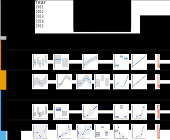
\includegraphics[width=170mm]{../../figures/model_descriptions} 

}

\caption{Summary of models fit to the West Coast Groundfish Observer Program bycatch dataset. The ratio estimator was stratified by Year, Bimonthly period, and Depth (fathoms). The Delta and Total models were fit to the same covariates, meant to mimic the stratified ratio estimator. Covariates treated as factors are indicated by \textit{fac}(). The Delta models split the bycatch data into presence/absence (Y) and positive catches (Z), then calculate bycatch as Y x Z. The Nonlinear models incorporate all available covariates using nonlinear terms, e.g. spline terms in GAMs, \textit{s}(). Covariate effect plots are shown for models fit to Pacific Hake bycatch (see Supplement for 14 other species and complete model statistics). We used the following R packages: 'mgcv' to fit GAMs, 'visreg' to visualize GAM covariate effects, 'randomForest' to fit RFs, and 'forestFloor' to visualize RF covariate effects.}\label{fig:model-descriptions}
\end{figure}

\pagebreak

\begin{figure}

{\centering \includegraphics[width=6in]{../../figures/fig2_effort_bycatch/fig2_effort_bycatch_caterpillar} 

}

\caption{Estimated relationships between fishing effort, defined as haul duration (hours, left panel) or catch of target species (kg, right panel), and bycatch for 15 species analyzed in the West Coast groundfish trawl fishery. The slope terms, $\beta$, of log-log linear models are exponents of an assumed power law fit to each species, $\text{Bycatch} = \alpha \text{Effort}^{\beta}$, with 95\% CIs shown for each estimate. Most $\beta$ are much less than 1 (left of dashed line), indicating the relationship between bycatch and effort is either weak or less-than-linear. Data ($n = 35,440$) consist of observed hauls from the West Coast Groundfish Observer Program recorded from 2011 to 2015 in the area north of Cape Falcon, Oregon (45.77° N).}\label{fig:effort-bycatch-slopes}
\end{figure}

\pagebreak

\begin{figure}

{\centering \includegraphics[width=6in]{../../figures/fig2_effort_bycatch/fig2_effort_bycatch_target_nozeros} 

}

\caption{Relationship between fishing effort (catch of target species in kg) and bycatch (kg) of 15 selected species in the West Coast groundfish trawl fishery. The slope terms, $\beta$, of log-log linear models are exponents of an assumed power law fit to each species, $\text{Bycatch} = \alpha \text{Effort}^{\beta}$. All $\beta$ are much less than 1, indicating the relationship between Bycatch and Effort is either weak or less-than-linear. Each data point ($n = 35,440$) is an observed haul from the West Coast Groundfish Observer Program recorded from 2011 to 2015 in the area north of Cape Falcon, Oregon (45.77° N).}\label{fig:effort-bycatch}
\end{figure}

\pagebreak

\begin{figure}

{\centering \includegraphics{bycatch_sim_paper_sepsupp_files/figure-latex/model-comparison-1} 

}

\caption{Predictive performance of the ratio estimator (status quo) and two spatial modeling frameworks: generalized additive models (GAMs) and random forests (RFs). We fit each model to 200 'training' datasets simulated with 20\% observer coverage, then predicted bycatch in unobserved hauls to calculate annual estimates of fleet-wide bycatch. We calculated model performance (RMSE) using the true, observed bycatch. For each species, the dashed line indicates the median RMSE for the ratio estimator, and solid lines indicate median RMSE for each model. GAM-Nonlinear clearly outperformed GAM-Delta and GAM-Total, which had convergence issues for 3/15 species. The RF models all performed similarly and had higher accuracy than the ratio estimator for all species, on average having 26\% lower RMSE (RF = 0.16, Ratio = 0.22).}\label{fig:model-comparison}
\end{figure}

\pagebreak

\begin{landscape}
\begin{figure}

{\centering 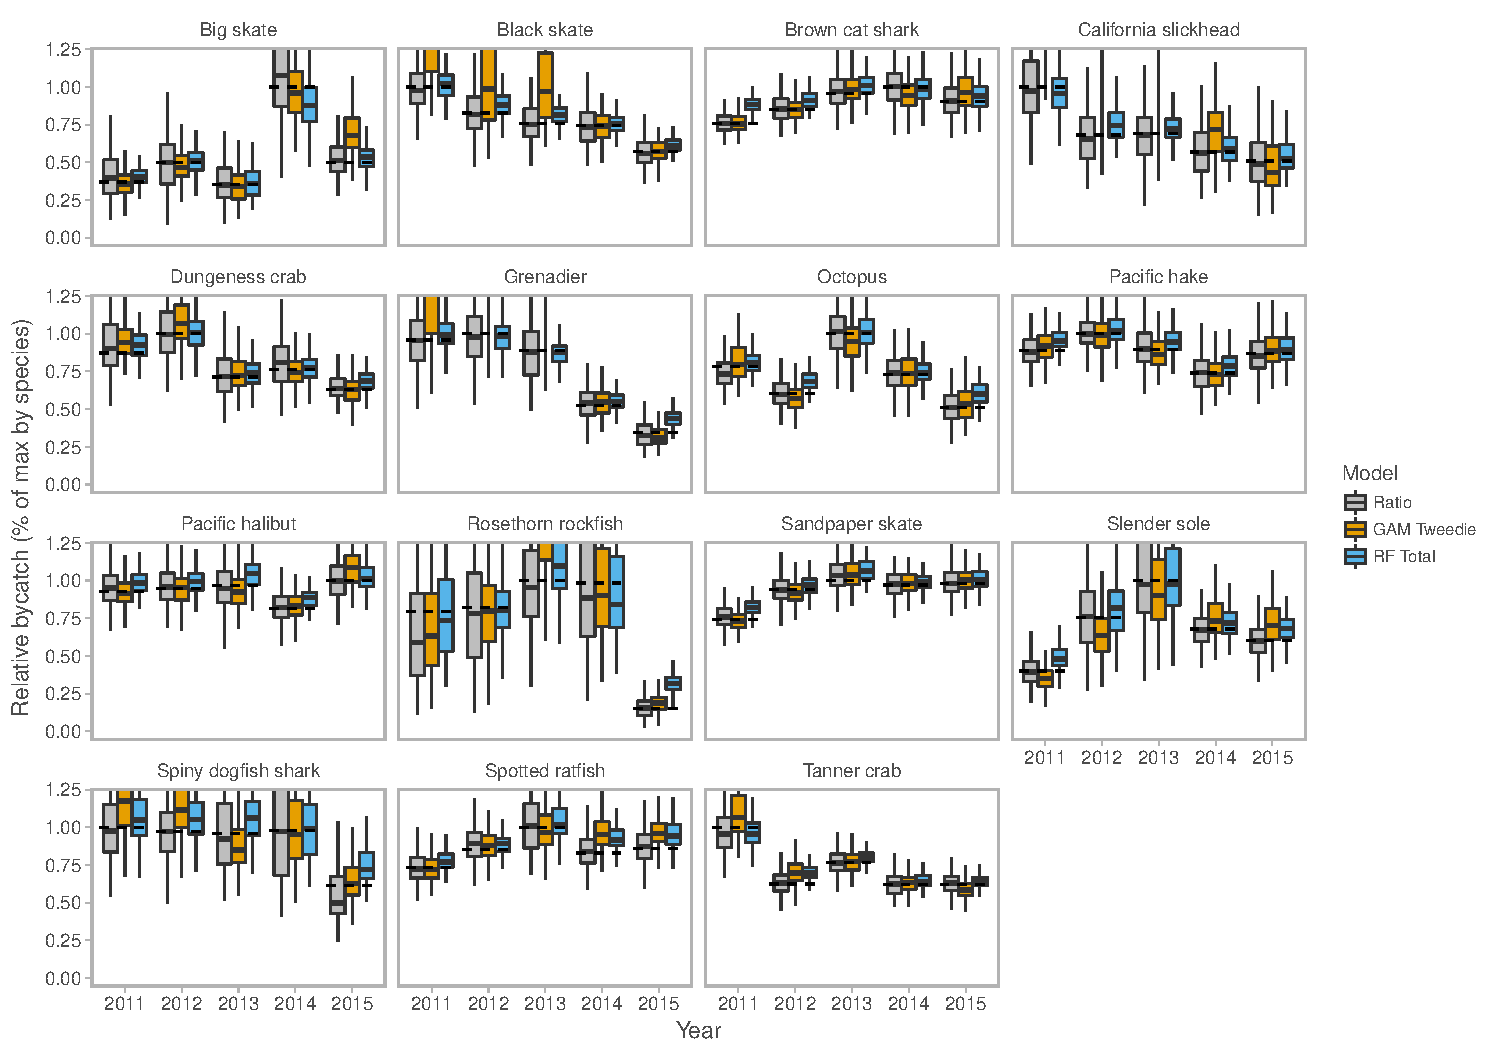
\includegraphics[width=10in]{bycatch_sim_paper_sepsupp_files/figure-latex/model-comparison-byyear-catch-1} 

}

\caption{Predictive performance of the ratio estimator (status quo) and two spatial modeling frameworks: generalized additive models (GAMs) and random forests (RFs). We fit each model to 200 'training' datasets simulated with 20\% observer coverage, then predicted bycatch in unobserved hauls to calculate annual estimates of fleet-wide bycatch. For each species and year, the dashed lines indicate the true observed bycatch. RF estimates were more precise (less variable) but also more biased. RF bias was generally positive, especially in years with below average bycatch (e.g. 2015 for most species).}\label{fig:model-comparison-byyear-catch}
\end{figure}
\end{landscape}

\pagebreak

\begin{figure}

{\centering \includegraphics[width=6in]{bycatch_sim_paper_sepsupp_files/figure-latex/model-comparison-byyear-1} 

}

\caption{Percent error of annual bycatch predictions using the ratio estimator (status quo), GAMs, and random forests (RFs), averaged across 15 species in the West Coast groundfish trawl fishery. Averaged across species, RF-Nonlinear was the most precise model, followed by GAM-Nonlinear and the ratio estimator (median absolute percent error: RF = 0.121, GAM = 0.131, Ratio = 0.155). While the ratio estimator was unbiased, the two spatial model-based estimators exhibited positive bias, particularly RF (median percent error: RF = 0.078, GAM = 0.026, Ratio = -0.002). We fit each model to 200 'training' datasets simulated with 20\% observer coverage, then predicted bycatch in unobserved hauls to calculate annual estimates of fleet-wide bycatch for each species. Percent error was calculated using the true, observed bycatch in each year.}\label{fig:model-comparison-byyear}
\end{figure}

\pagebreak

\begin{figure}

{\centering \includegraphics[width=6in]{../../figures/supplement/fig10_bycatch_rate_rmse} 

}

\caption{RF reduction in prediction error compared to the ratio estimator, as a function of bycatch rate for 15 species in the U.S. West Coast groundfish trawl fishery. RF improved on the ratio estimator for all species (26\% lower RMSE on average), but this improvement was greater for species with lower bycatch rates (e.g. Rosethorn rockfish, California slickhead, Big skate, Black skate, Dungeness crab, Grenadier).}\label{fig:bycatch-rate-rmse}
\end{figure}

\pagebreak

\begin{figure}

{\centering \includegraphics[width=6in]{../../figures/supplement/fig7_tradeoffs_v2} 

}

\caption{Bias-variance trade-off between the ratio estimator and RF. RF achieves more accurate predictions (lower RMSE) by allowing some bias but greatly reducing the variance of its estimates. The ratio estimator has very low bias but much higher variance (i.e. it underfits the data and is more sensitive to which hauls are observed). Dashed grey lines indicate iso-RMSE curves. Species with lines that are nearly parallel to the iso-RMSE curves (e.g. Octopus, Brown cat shark) indicate that RF and the ratio estimator perform similarly (same RMSE). Species with lines that cross iso-RMSE curves (e.g. Dungeness crab, California slickhead, Spiny dogfish shark) indicate RF greatly improves on the ratio estimator (lower RMSE). RF has lower RMSE for species with lower bycatch rates (Fig. 8).}\label{fig:variance-bias}
\end{figure}


\end{document}
